\chapter{CountMax的应用}


\section{借助CountMax进行重路由}\label{sec:flowrerouting}
流的重路由对于许多实际应用都是必要且十分重要的,如链路负载均衡以及链路中断时的重新寻路\cite{xu2017incremental}
。对于这些应用,网络中的大流的流量统计信息更加重要\cite{xu2017scalable}。

通过周期性地收集交换机的统计数据,控制器可以监控链路的流量负载。当控制器发现某条链路负载过重时,就需要对流进行重路由。
如果在交换机上安装了CountMax,控制器就可以收集CountMax中的信息,从而找出大流的集合,记为 $\Gamma^e$。
由于大流的流量占据了了网络整体流量中的大部分,因此通过采用各种算法对这些大流进行重路由,就可以快速有效地优化链路负载。
例如,我们可以利用一个简单的贪心法来重路由这些大流。首先将大流按照流量降序排列,然后按照顺序,控制器对每条流寻找一个占用率最低的路径作为新的路由。
在为所有大流都找好了新路径之后,将这些路径下发到交换机中\cite{jin2014dynamic} \cite{xu2017joint}。

这一过程中只对大流进行了重路由,而大流的数量和网络中流的总数相比非常少,因此重路由所需的时间也大幅减少。
由于CountMax的存储占用很小,因此收集CountMax的信息也不会为控制器带来明显的负载。


% \section{近似性能和计算负载的初步模拟}
% 小节\ref{sec:analysis}中的分析当中多次使用了不等式缩放、马尔可夫不等式,因此最终得到的结论颇为宽松。
% 为了更清楚的了解CountMax的实际性能,我们用C语言实现了CountMax并进行了一系列模拟。关于模拟环境的详细介绍请参见第XXXX章。
\begin{figure}[!h]
	\centering
	\begin{minipage}[t]{0.48\linewidth}		
		%\begin{figure}[!t]
		\centering
		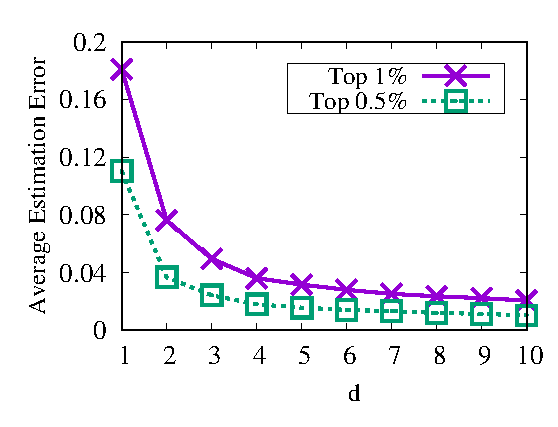
\includegraphics[width=\linewidth]{fig/cm_d_err.eps}
		\caption{\textnormal{CountMax近似误差与$d$的关系}}
		\label{fig:cm,d,acc}
		%\end{figure}
	\end{minipage}\vspace{-0.6em}
\hspace{0.4em}
	\begin{minipage}[t]{0.48\linewidth}
        \centering
		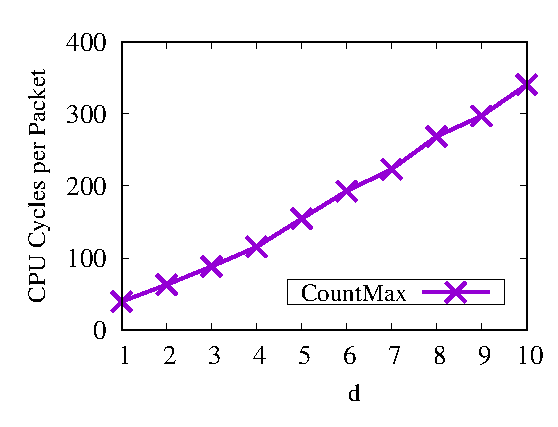
\includegraphics[width=\linewidth]{fig/cm_d_cpu.eps}
		\caption{\textnormal{CountMax处理一个数据包的平均CPU周期数}}
		\label{fig:cm,d,cpu}
	\end{minipage}\vspace{-0.6em}
\hspace{0.1em}
\end{figure}

\section{CountMax的协作式部署}\label{sec:coop}
要进一步降低CountMax在交换机上的计算负载,主要有两种方法。第一种方法是通过减少$d$的值,也就是CountMax的行数。

图\ref{fig:cm,d,acc}描述了CountMax在不同的行数下,对网络中前1\%或0.5\%的流的流量估计的误差。
关于测试环境的具体介绍请参见第XXXX章。图\ref{fig:cm,d,acc}中的测试对应的是其中Spine-Leaf拓扑、20万条流、$k=2000$、非协作式的情况。
由图中我们可以看到,随着$d$的增长,估计误差一开始迅速降低,但随后降低的速度大幅放缓。$d=3$时的误差和$d=10$时的误差差别很小。
当$d=2$时,误差已经控制在10\%以内。

图\ref{fig:cm,d,cpu}描述了CountMax处理数据包所需的CPU时钟周期随$d$的变化而变化的情况。
图中的结果显示,CountMax的处理一个包的计算负载和$d$大致呈线性增长,同时印证了定理\ref{tm:time}。


\begin{figure}[h]
   \centering
   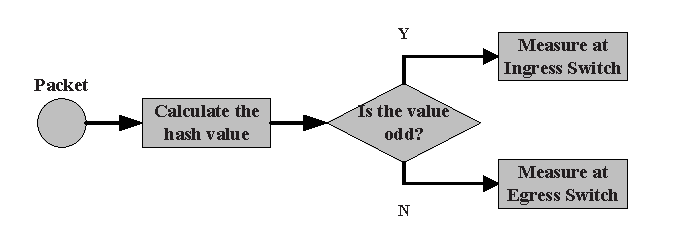
\includegraphics[width=\linewidth]{fig/filter_measure.eps}
   \caption{Illustration of the Cooperative Measurement Framework}
   \label{fig:filtermeasurement}
\end{figure}

另一种降低计算负载的方法是减少CountMax所需要处理的数据包的个数。要测量流的流量,最简单的方案就是在每一个交换机上都部署一个CountMax,并且处理经过交换机的所有数据包。
然而,网络中的很多流是要经过多个交换机的(由于CountMax的主要应用是流的重路由,所以实际上我们只关心那些要经过多个交换机的流),同一条流可能会被多个交换机统计,造成资源的浪费。

因此,本文提出了一种“协作”的方法,让一条流只会被一个交换机测量。协作式的流量测量的流程如图\ref{fig:filtermeasurement}所示。
每当一个数据包抵达交换机时,交换机首先用一个哈希函数对流的ID进行哈希。这个哈希函数是所有交换机所共享的。
如果哈希的结果是奇数,那么这条流应当被它的入口交换机,也就是路由上的第一个交换机进行测量。反之则被出口交换机所测量。
交换机可以通过这条流的入端口和出端口来判断自己是不是入口交换机或者出口交换机。

接下来分析协作式CountMax的估计误差。不失一般性,我们假设网络中只有两个交换机。网络中的所有流都是先经过交换机1,再经过交换机2的。
假设所有流的总流量是$F$,交换机1处理的流量占比是$\gamma_1 $,那么它处理的总流量就是$F_1 =\gamma_1\cdot F $。
相应的,交换机2处理的流量占比是$\gamma_2 $,总流量是$F_2 =\gamma_2\cdot F $。

首先关注交换机1。令$f$代表网络中所有的流当中的一条$\delta$-heavy hitter流,则$f$的流量大于$\delta \cdot F$。
如果$f$是被交换机1所处理的,那么对于被交换机所处理的流的集合而言,$f$是一个$\delta/\gamma_1$-heavy hitter。
根据定理\ref{tm:query}和定理\ref{tm:acc},有如下不等式成立:

\begin{equation}\label{eq:coop_acc}
\left\{
\begin{aligned}
&Pr[1-\frac{e\cdot \gamma_x}{w\cdot \delta}\le \frac{\hat{a}_i}{a_i} \le 1] \ge 1-e^{-\tilde{d}}\\
&E[\tilde{d}]\ge d\cdot(1-\frac{\gamma_x}{w\cdot\delta})
\end{aligned}
\right.
\end{equation}

其中$\gamma_x$ 根据这条流被哪个交换机所测量,而代表 $\gamma_1$ 或 $\gamma_2$。如果定义 $\gamma_m = \max \{\gamma_1, \gamma_2\}$,用$\gamma_m$替换$\gamma_x$,即可得到一个下界。在最好的情况下,$\gamma_1=\gamma_2=1/2$。在实际情况中,通过选择足够随机的哈希函数,$\gamma_1$ 和 $\gamma_2$通常都会比较接近。参照等式\eqref{eq:coop_acc}, 协作式CountMax将$\frac{\hat{a}_i}{a_i}$ 和 $E[\tilde{d}]$ 这两个值的界缩紧为原本的 $\gamma_m $倍。





%\section{CountMax-Based Hierarchical Heavy Hitters (HHH)}

%If a flow $f$ has destination host of IP address 10.11.12.13, it has different keys in different levels. For the 1st level the key of $f$ is 10.0.0.0, for the 2nd level it's 10.11.0.0, and so on.

%As an extension of Heavy Hitters, Hierarchical Heavy Hitters (HHH) is to find out the heavy hitters in different levels of a hierarchical model. For example, we can classify flows according to subnets of the destination host, and there can be multi levels of subnets. More specificity, suppose there are 4 levels, denoted by level 0 to level 3, and the subnet mask is 255.255.255.255 for level 0, 255.255.255.0 for level 2, and so on. For level 0, it directly deals with flows; For higher levels, they deal with sets of flows, according to the subnets that flows belong to. Given a threshold $\delta$, for level 0, the hierarchical heavy hitters are just the heavy hitter flows. For the $i$th level ($i>0$), it's a bit more complex.

%As mentioned before, the higher levels deal with flow sets instead of flows. For the $i$th level ($i>0$), the weight of a flow set $s$ is defined as the sum of traffic of flows, where each flow satisfies: the flow belongs to $s$, but does not belong to any HHH of lower levels.

%Authors of \cite{cheung2006finding} have discussed the implementation of general HHH based on Count-Min. However, Count-Min cannot find out HHH flows since it doesn't record flow keys. Suppose that there are $g$ levels of hierarchies. To solve the HHH problem, we need to keep $g$ CountMax sketches, denoted by $C_1, ... ,C_g$, where $C_i$ corresponds the $i$th hierarchical level from top to bottom.

%When a packet arrives, for every level $i \in \{1, ..., g\}$, we first calculate the level-specified key $key_{i}$. In the previous example, if a flow $f$ has destination host of IP address 10.11.12.13, its $key_0$ is 10.11.12.13, $key_1$ is 10.11.12.0, $key_2$ is 10.11.0.0, and $key_3$ is 10.0.0.0. Then we update $C_{i}$ using $key_{i}$ as the key. To find out heavy hitters of every hierarchy level, we just iterate the CountMax sketches from $C_g$ to $C_1$, and figure out the result according to the definition of HHH.

